\documentclass[10pt,a4paper]{article}
\usepackage[utf8]{inputenc}
\usepackage[T1]{fontenc}
\usepackage{amsmath,amssymb}
\usepackage{booktabs}
\usepackage{graphicx}
\usepackage{xcolor}
\usepackage{hyperref}
\usepackage[margin=2.2cm]{geometry}
\usepackage{caption}
\usepackage{subcaption}
\usepackage{parskip}
\usepackage{enumitem}
\usepackage{array}
\usepackage{multicol}
\usepackage{fancyhdr}
\usepackage{titlesec}
\usepackage{tcolorbox}
\usepackage{microtype}

\hypersetup{colorlinks=true, linkcolor=blue!70!black, citecolor=blue!70!black, urlcolor=blue!70!black}

% Section formatting
\titleformat{\section}{\large\bfseries\color{blue!60!black}}{}{0em}{}[\titlerule]
\titleformat{\subsection}{\normalsize\bfseries\color{blue!40!black}}{}{0em}{}
\setlength{\parskip}{4pt}

% Header/footer
\pagestyle{fancy}
\fancyhf{}
\rhead{\small NIFE/IKM Internal Report}
\lhead{\small Dieckow Analysis Summary}
\cfoot{\small \thepage}

% Color boxes
\tcbuselibrary{skins}
\newtcolorbox{keybox}[1][]{colback=blue!5!white, colframe=blue!50!black,
  fonttitle=\bfseries, title=#1, left=4pt, right=4pt, top=3pt, bottom=3pt}
\newtcolorbox{jabox}[1][]{colback=orange!5!white, colframe=orange!50!black,
  fonttitle=\bfseries, title=#1, left=4pt, right=4pt, top=3pt, bottom=3pt}
\newtcolorbox{limitbox}[1][]{colback=red!5!white, colframe=red!40!black,
  fonttitle=\bfseries, title=#1, left=4pt, right=4pt, top=3pt, bottom=3pt}

\newcommand{\bphi}{\boldsymbol{\phi}}
\newcommand{\bA}{\mathbf{A}}
\newcommand{\bb}{\mathbf{b}}

% ─────────────────────────────────────────────────────────────────────
\title{%
  \textbf{Summary Report}\\[4pt]
  \large Metabolic-Prior Replicator Dynamics Predict Oral Microbiome\\
  Community Composition under Leave-One-Out Cross-Validation\\[6pt]
  \normalsize \textit{NIFE/IKM Internal Analysis — Nishioka \& Szafra\'{n}ski, \today}
}
\author{}
\date{}

\begin{document}
\maketitle\thispagestyle{fancy}
\vspace{-1em}

% ═══════════════════════════════════════════════════════════════════════
\begin{tcolorbox}[colback=gray!8, colframe=gray!50, title=\textbf{Abstract / 要旨}]
\begin{multicols}{2}
\small
\textbf{[English]}
We test whether metabolic network constraints from flux-balance analysis (FBA)
can improve out-of-sample prediction of oral microbiome dynamics.
A Hamilton replicator ODE with a three-layer metabolic sign prior
(eHOMD + AGORA2) was fit to 16S rRNA time-series data from 10 patients
(Dieckow et~al.~2024).
Leave-one-patient-out (LOO) cross-validation shows:
\textbf{LOO-RMSE = 0.050 $\pm$ 0.021} (AGORA W=1.0),
\textbf{LOO Bray-Curtis = 0.147} (48\% below persistence null).
External validation on 127 peri-implant samples confirms dysbiosis ordering
($p < 0.0001$).

\columnbreak

\textbf{[日本語]}
代謝ネットワーク制約（フラックスバランス解析: FBA）が経口マイクロバイオームの
予測を改善するかを検証した。
10名の患者データ（Dieckow 2024）に対し、代謝的サインプライアを組み込んだ
Hamilton Replicator ODEをフィット。
LOO交差検証の結果：
\textbf{LOO-RMSE = 0.050 $\pm$ 0.021}（AGORA W=1.0）、
\textbf{LOO Bray-Curtis = 0.147}（持続性ヌルモデル比 $-$48\%）。
127例の独立インプラント周囲炎サンプルでの外部検証でも
Dysbiosis順序付けを再現（$p < 0.0001$）。
\end{multicols}
\end{tcolorbox}

% ═══════════════════════════════════════════════════════════════════════
\section{1. Background \& Motivation \quad /\quad 背景と動機}

\begin{multicols}{2}
\small
\textbf{[EN]}
Oral microbiome communities are spatially structured syntrophic systems underlying
dental caries and periodontal disease.
Longitudinal 16S rRNA data provide time snapshots, but the generalised Lotka-Volterra
(gLV) interaction matrix $\bA$ is severely underdetermined
($K^2 \sim 100$ parameters, $N{=}10$ patients $\times$ 3 timepoints).
Standard $L_2/L_1$ regularisation treats all interactions equally;
a biologically motivated approach constrains the \emph{sign} of $A_{ij}$ via known
metabolic cross-feeding.

\textbf{This study:} Three-layer sign prior (L1: eHOMD experimental flows,
L2+L3: AGORA2 pFBA), combined with the Hamilton replicator (symmetric $\bA$)
and JAX autodiff optimisation, applied to Dieckow et~al.~(2024).

\columnbreak

\textbf{[日本語]}
経口マイクロバイオームは歯周病・う蝕の病態基盤となる合成栄養コミュニティ。
16S rRNAの縦断データで相互作用行列 $\bA$ を同定するが、
パラメータ数（$\sim$100）に対してデータが少なく（10名×3週）、
正則化が必須。

通常のリッジ/LASSO は全相互作用を同等に扱うが、
FBAや実験データから得られる代謝的「符号制約」は生物学的に根拠がある。

\textbf{本研究:} 3層サインプライア（L1: eHOMD実験データ、L2+L3: AGORA2 pFBA）と
Hamilton Replicator（対称 $\bA$）を組み合わせ、Dieckow 2024データに適用。
\end{multicols}

% ═══════════════════════════════════════════════════════════════════════
\section{2. Methods \quad /\quad 手法}

\begin{multicols}{2}
\small
\textbf{Dataset:} Dieckow et~al.~(2024), 10 patients (A--H, K, L),
subgingival plaque on titanium implant abutments, 3 weekly timepoints.
Aggregated to 10 class-level guilds (Actinobacteria, Bacilli, Bacteroidia,
Betaproteobacteria, Clostridia, Coriobacteriia, Fusobacteriia,
Gammaproteobacteria, Negativicutes, Other).

\textbf{Model — Hamilton Replicator:}
\[
  \dot\phi_i = \phi_i(f_i - \bar f),\quad f_i = b_i + \textstyle\sum_j A_{ij}\phi_j
\]
Symmetric $A_{ij}=A_{ji}$, $A_{ii}<0$. RK45 integration (JAX-JIT).

\textbf{Sign prior:}
\begin{itemize}[noitemsep,leftmargin=*]
  \item \textbf{L1}: eHOMD/Szafra\'{n}ski experimental metabolite flows (34 pairs, $w=2.0$)
  \item \textbf{L2}: AGORA2 pFBA cross-feeding (adds 1 pair, $w=1.0$)
  \item \textbf{L3}: Additional AGORA signals at swept weight $w\in[0.5,2.0]$
\end{itemize}
Hinge-squared penalty: $\mathcal{P} = \sum_{ij}\frac{|F_{ij}|}{2\sigma^2}[\max(0,-\text{sgn}(F_{ij})A_{ij})]^2$,
$\sigma=0.15$.

\textbf{Optimisation:} L-BFGS-B, JAX autodiff, 5000 iterations.
LOO: fix $\bA$, re-optimise $\hat b^{(p)}$ from W1 only.

\columnbreak

\textbf{データ:} Dieckow 2024, 10名、チタンインプラントアバットメント上の
縁下プラーク、週1回×3週。10ギルド（クラスレベル）に集約。

\textbf{Hamilton Replicatorモデル:}
\[
  \dot\phi_i = \phi_i(f_i - \bar f),\quad f_i = b_i + \textstyle\sum_j A_{ij}\phi_j
\]
対称 $A_{ij}=A_{ji}$（Hamilton原理から自然に要請）、$A_{ii}<0$。

\textbf{サインプライア:}
\begin{itemize}[noitemsep,leftmargin=*]
  \item \textbf{L1}: eHOMD/Szafra\'{n}ski実験的代謝フロー（34ペア）
  \item \textbf{L2}: AGORA2 pFBA 相互栄養（1ペア追加）
  \item \textbf{L3}: AGORA重み $w$ をスイープ
\end{itemize}
ヒンジ2乗ペナルティで符号違反をペナルティ化。$\sigma=0.15$。

\textbf{最適化:} L-BFGS-B + JAX自動微分、5000回。
LOO: $\bA$ を固定し、W1データのみで $\hat b^{(p)}$ を再最適化。

\textbf{評価指標:} LOO-RMSE（二乗平均誤差）+ Bray-Curtis非類似度（生態学的標準）。
\end{multicols}

% ═══════════════════════════════════════════════════════════════════════
\section{3. Key Results \quad /\quad 主要結果}

\subsection{3.1 LOO Cross-Validation Performance \quad /\quad LOO交差検証}

\begin{table}[h]
\centering
\small
\caption{LOO cross-validation comparison (best values \textbf{bold}). /
LOO交差検証の比較（太字が最良値）。}
\begin{tabular}{llcccc}
\toprule
Model & Prior & SA (\%) & LOO-RMSE & Std & LOO-BC \\
\midrule
gLV free (asymm.)        & None     & ---     & 0.0588 & ---   & 0.154 \\
Hamilton (no prior)      & None     & ---     & 0.0595 & 0.024 & ---   \\
Hamilton L1+L2           & L1+L2    & 94      & 0.0516 & 0.021 & 0.155 \\
\textbf{Hamilton AGORA W1.0} & \textbf{L1+L2+L3} & \textbf{100} & \textbf{0.0504} & \textbf{0.021} & \textbf{0.147} \\
Persistence null         & ---      & ---     & ---    & ---   & 0.281 \\
Grand-mean null          & ---      & ---     & ---    & ---   & 0.254 \\
\bottomrule
\end{tabular}
\end{table}

\begin{keybox}[Key Numbers / 数値まとめ]
\begin{multicols}{2}
\small
\begin{itemize}[noitemsep]
  \item LOO-RMSE: \textbf{0.0504} (AGORA W1.0) vs. 0.0588 (gLV) → $-$14.3\%
  \item LOO-BC: \textbf{0.147} vs. 0.281 (persistence) → $-$47.7\%
  \item Sign agreement: \textbf{70/70 (100\%)} at W=1.0
  \item 7/10 patients improve with AGORA prior
  \item Paired $t$-test: $p=0.08$ (marginal, $N=10$)
\end{itemize}
\columnbreak
\begin{itemize}[noitemsep]
  \item AGORAプライア（W1.0）でgLV比 $-$14.3\% RMSE改善
  \item 持続性ヌル比 $-$47.7\% Bray-Curtis改善
  \item 符号一致率: W=1.0で70/70 \textbf{100\%}
  \item 10患者中7名で改善
  \item 対応t検定: $p=0.08$（$N=10$で有意水準直前）
\end{itemize}
\end{multicols}
\end{keybox}

\subsection{3.2 Interaction Matrix \& Biological Regimes \quad /\quad 相互作用行列と生態学的解釈}

\begin{multicols}{2}
\small
\begin{figure}[H]
\centering
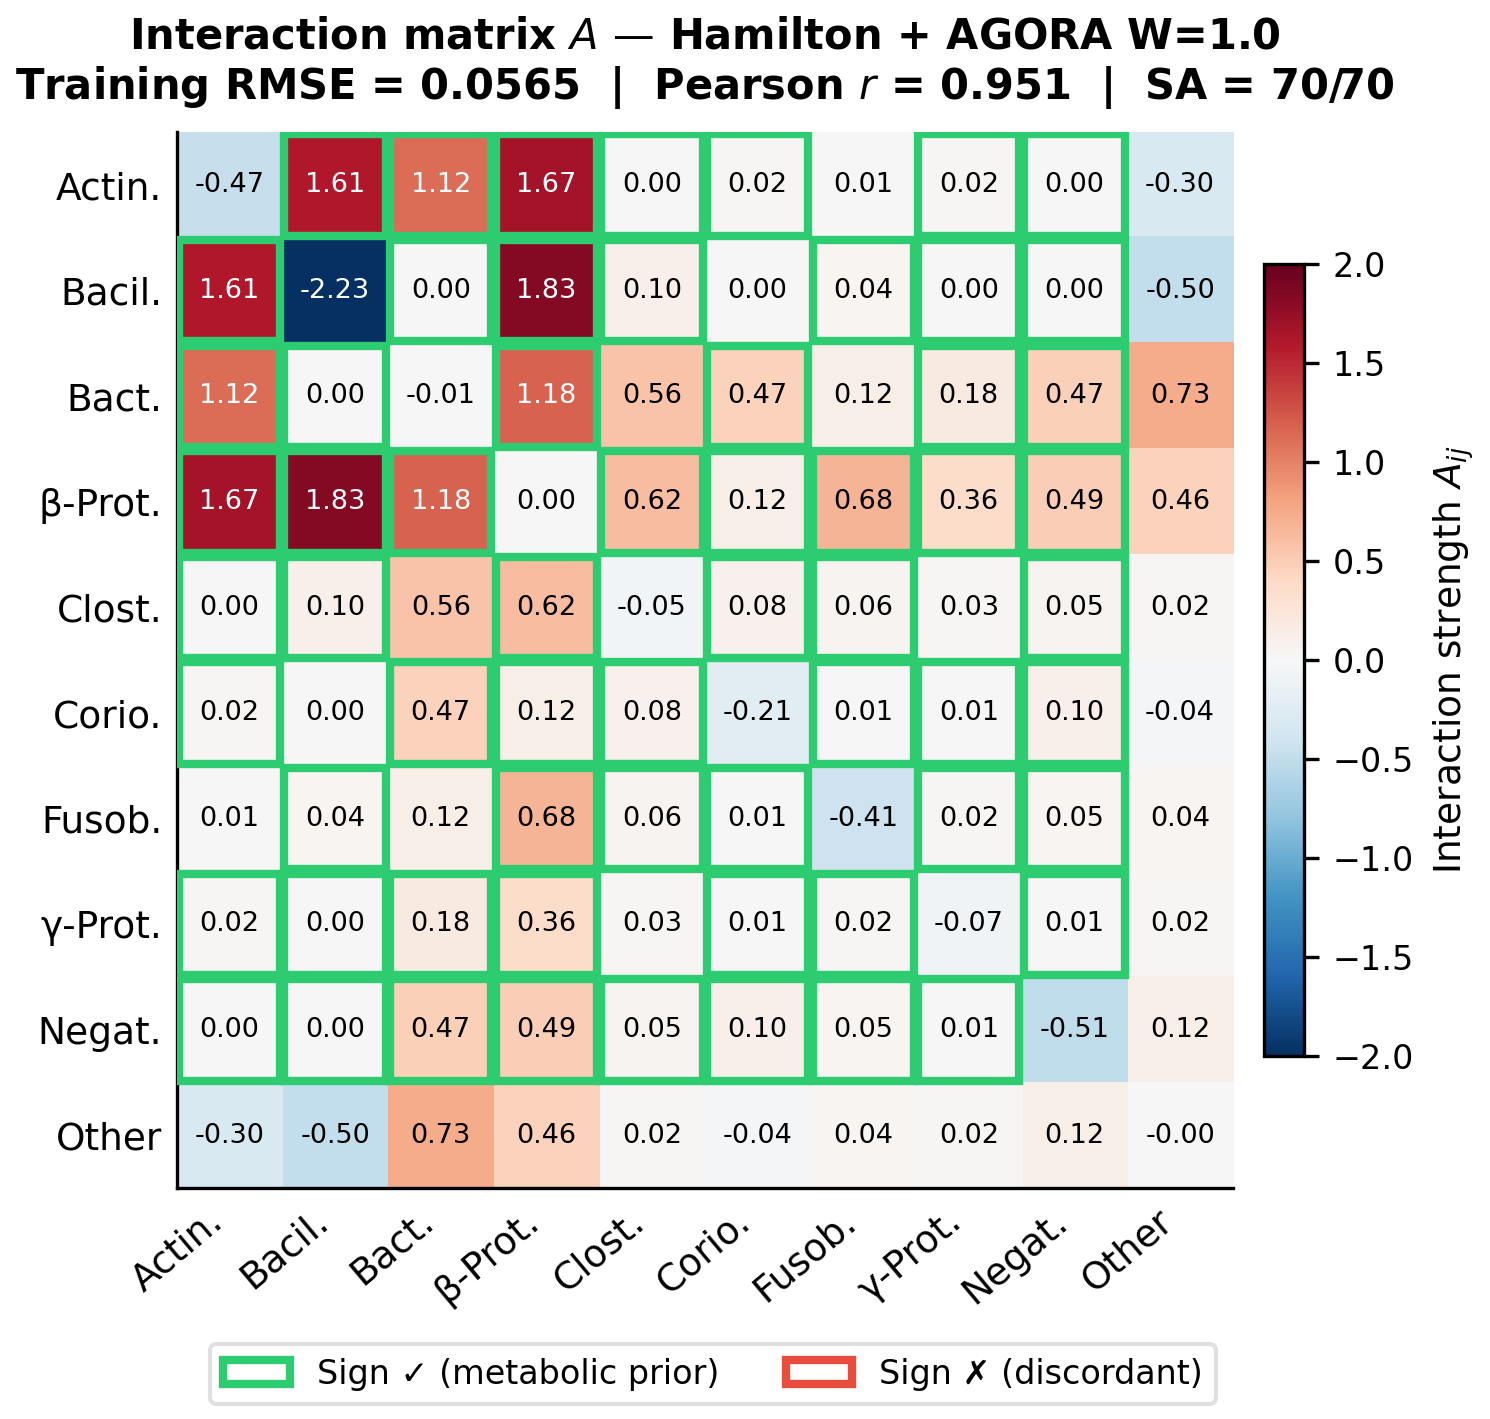
\includegraphics[width=0.95\linewidth]{figures/fig1_A_matrix.png}
\caption{\small Fitted $\bA$ matrix (AGORA W=1.0). Red = facilitation, Blue = competition.
All diagonal $A_{ii}<0$. Checkmarks = sign agrees with prior. /
フィットされた $\bA$（赤＝促進, 青＝競争）。全対角は負。チェック＝プライアと符号一致。}
\end{figure}
\columnbreak
\small
\textbf{Three ecological regimes / 3つの生態学的レジーム:}
\begin{enumerate}[noitemsep,leftmargin=*]
  \item \textbf{Data+Prior aligned (13 pairs):} Strong interactions confirmed
        by both data and metabolic evidence. Sign consistency SC=1.00 across all LOO folds.
        例: Actinobacteria--Bacilli ($A_{01}=+1.61$), co-aggregation文献と整合。
  \item \textbf{Prior-constrained, muted (22 pairs):} Strong FBA evidence,
        ecologically muted over 3 weeks.
        例: Bacilli--Negativicutes ($A=+0.003$, Streptococcus-lactate-Veillonella軸)。
  \item \textbf{Data-driven, no prior (10 pairs):} Ecological signal without
        metabolic annotation, concentrated around ``Other'' guild.
\end{enumerate}
\textbf{Key}: dominant facilitations among early commensals (Actinobacteria--Bacilli--Betaproteobacteria)
consistent with documented co-aggregation syntrophies.
\end{multicols}

\subsection{3.3 Community Structure \& Patient Clustering \quad /\quad コミュニティ構造}

\begin{multicols}{2}
\small
\begin{figure}[H]
\centering
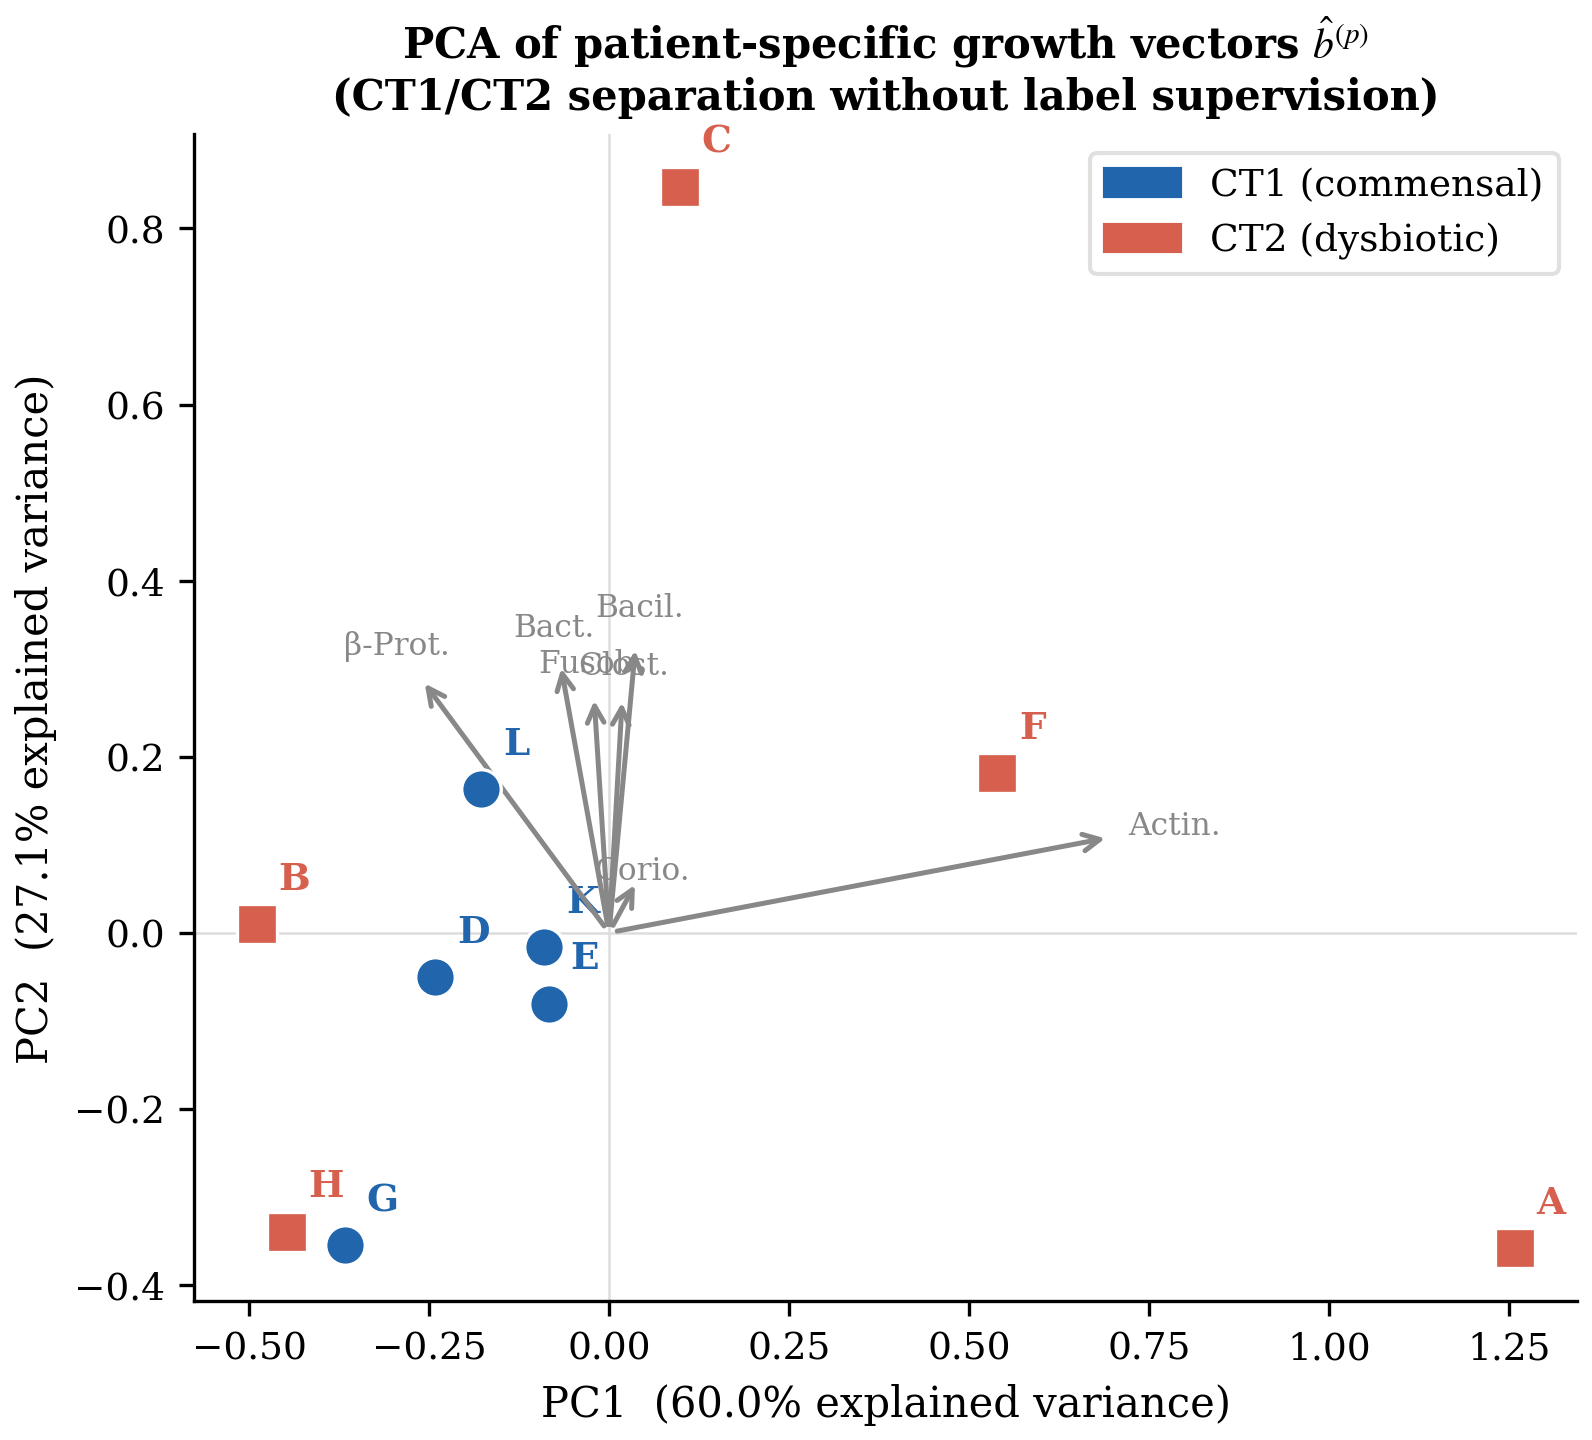
\includegraphics[width=\linewidth]{figures/fig4_b_pca.png}
\caption{\small PCA of patient-specific growth vectors $\hat{\bb}^{(p)}$.
PC1 separates CT1 (commensals) vs CT2 (dysbiotic) without supervision. /
成長ベクトル $\hat{b}$ のPCA。ラベルなしでCT1/CT2が分離。}
\end{figure}
\columnbreak
\small
\textbf{PCA/LDA ordination confirms:}
\begin{itemize}[noitemsep,leftmargin=*]
  \item Predicted compositions span the same manifold as observations
        (no regression-to-mean failure mode).
  \item LDA accuracy: \textbf{90\%} CT1/CT2 discrimination under LOO prediction.
  \item $\hat{\bb}^{(p)}$ PCA: CT1 vs CT2 separated by PC1 \emph{without supervision}.
  \item Mean $|A_\text{off-diag}|=0.35$ vs mean $|\hat{b}|=0.18$:
        community ecology dominates over individual growth rates.
\end{itemize}

\textbf{コミュニティ型:}
CT1（早期共生: Actinobacteria, Bacilli主体, 5名）vs
CT2（後期/Dysbiotic: Fusobacteriia, Bacteroidia主体, 5名）。
$\hat{b}$ のPC1がラベルなしで両者を分離 → 個体差は成長率に吸収される。
\end{multicols}

\subsection{3.4 External Validation: Peri-implant Dysbiosis \quad /\quad 外部検証}

\begin{multicols}{2}
\small
\begin{figure}[H]
\centering
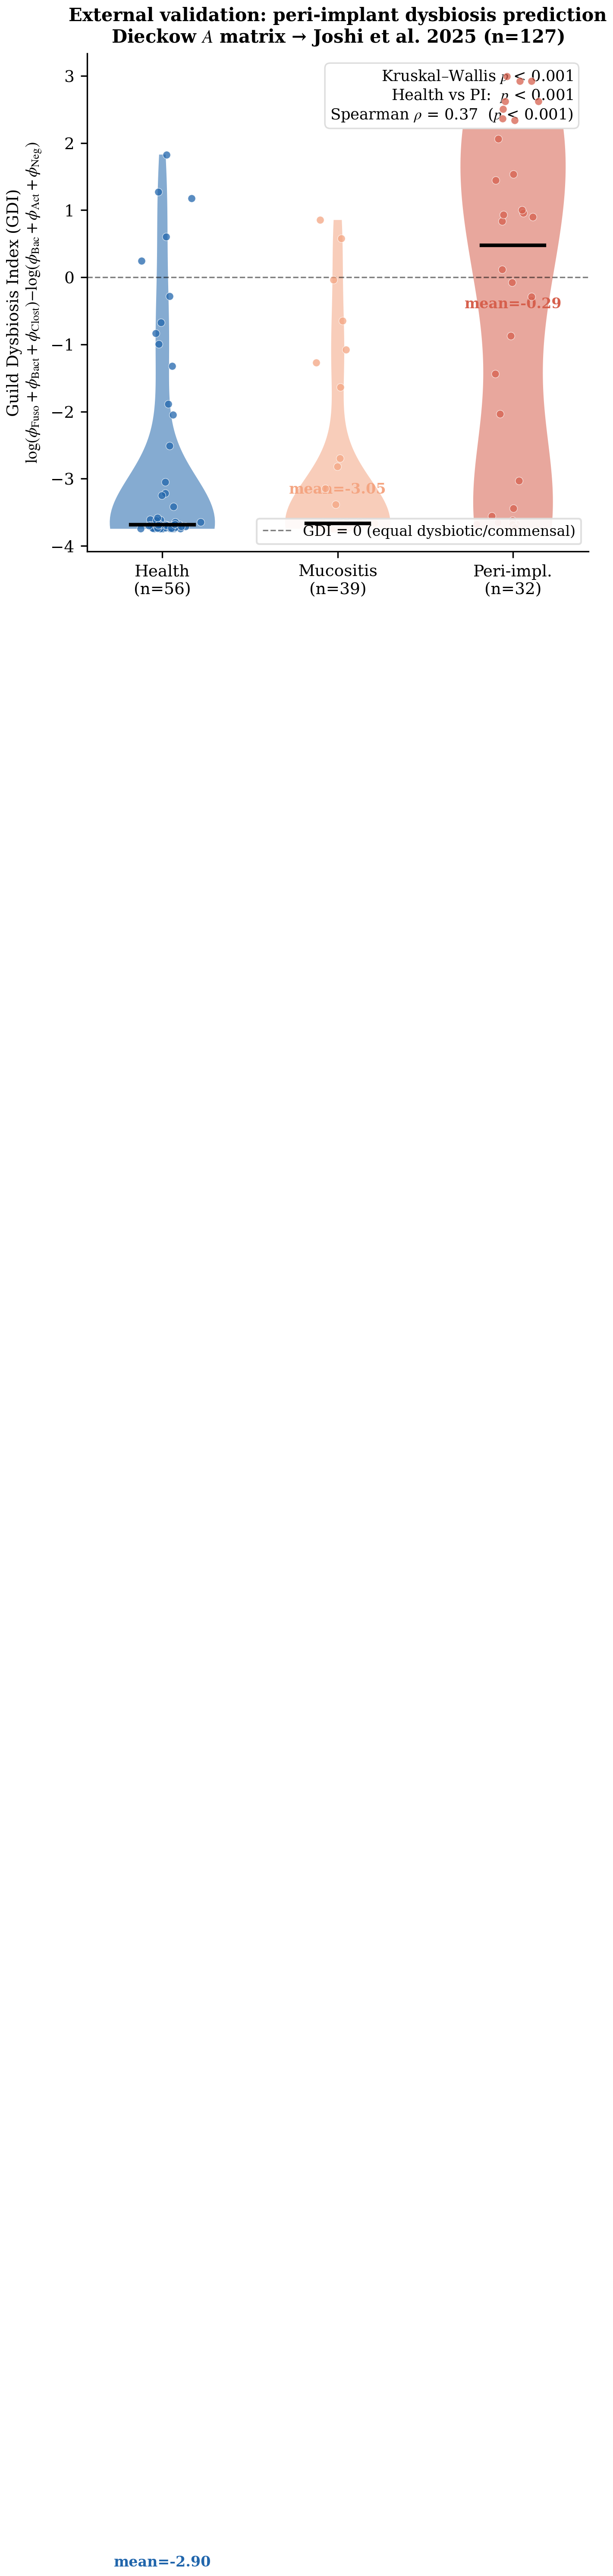
\includegraphics[width=0.95\linewidth]{figures/fig3_joshi_attractor.png}
\caption{\small guild-level R/G ratio in 127 peri-implant samples (Joshi 2025).
Peri-implantitis shifts significantly toward dysbiotic attractor. /
127例のR/G ratio分布。歯周炎群でDysbiotic側へ有意偏位。}
\end{figure}
\columnbreak
\small
\textbf{Joshi et~al.~2025 (127 cross-sectional samples):}
\begin{itemize}[noitemsep,leftmargin=*]
  \item Health: R/G ratio mean $= -2.90$
  \item Mucositis: R/G ratio mean $= -3.05$ ($p=0.61$ vs Health)
  \item Peri-implantitis: R/G ratio mean $= -0.29$ ($p < 0.0001$ vs Health)
  \item Kruskal-Wallis: $H=30.4$, $p<0.0001$
  \item Spearman $\rho = 0.37$ ($p < 0.0001$)
\end{itemize}

Dieckow $\bA$（10患者、3週間のキャリス回復データ）が、
全く独立した127例のインプラント周囲炎データで
Dysbiosis重症度を正しく順序付け。
アトラクタが $\bA$ のみで決定される理論的予測を実験的に支持。
\end{multicols}

% ═══════════════════════════════════════════════════════════════════════
\section{4. AGORA Phase Transition \quad /\quad AGORAの相転移}

\begin{multicols}{2}
\small
\begin{figure}[H]
\centering
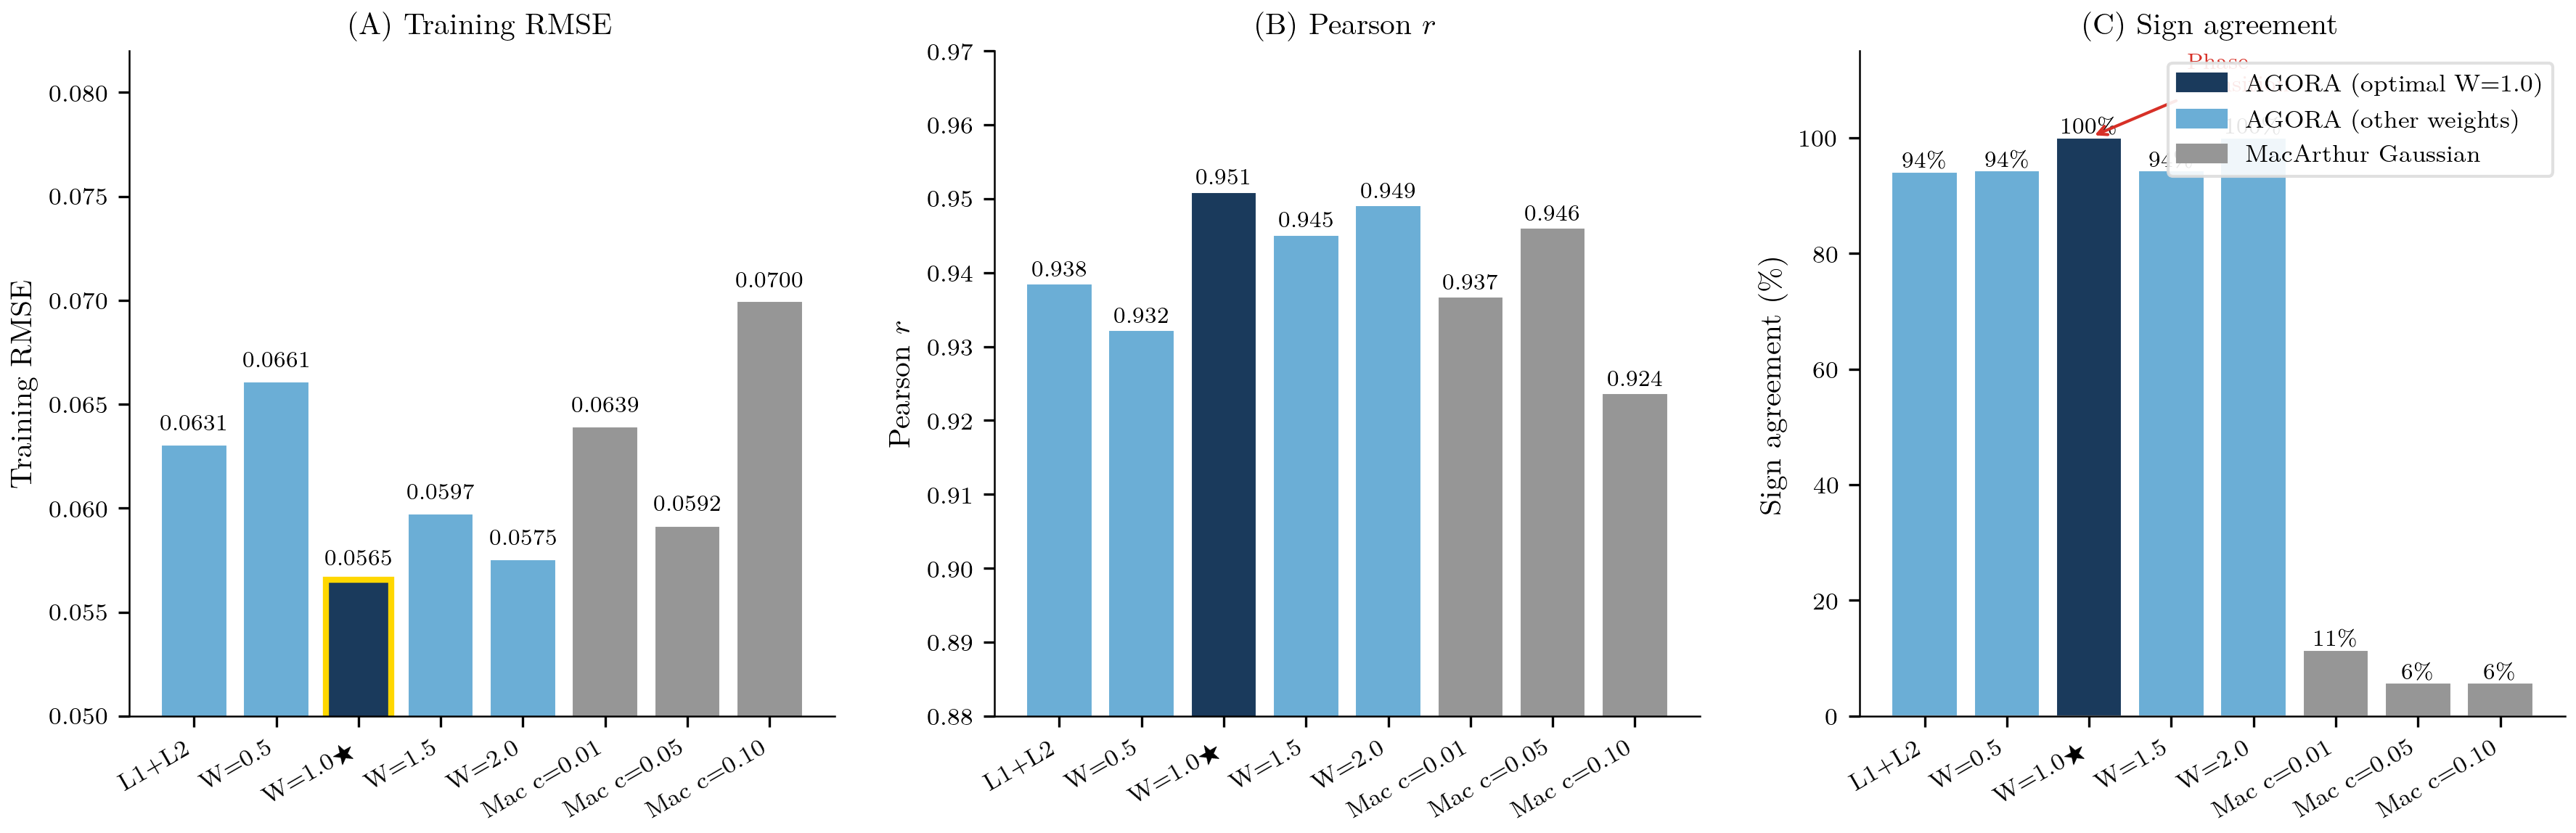
\includegraphics[width=0.95\linewidth]{figures/fig6_agora_weight_sweep.png}
\caption{\small AGORA weight sweep. Phase transition at $w=1.0$: SA jumps to 100\%
with simultaneous RMSE reduction. MacArthur Gaussian prior fails completely. /
AGORA重みスイープ。$w=1.0$ で相転移：SA 100\%、同時にRMSE最小。MacArthur型は完全失敗。}
\end{figure}
\columnbreak
\small
\textbf{Key finding / 重要な知見:}
FBAは相互作用の\textbf{符号}は予測できるが、\textbf{大きさ}は予測できない。

\begin{itemize}[noitemsep,leftmargin=*]
  \item $w=1.0$ で離散的相転移: SA 94\% → 100\%, RMSE同時最小
  \item $w>1.0$ ではSAが94\%に戻り過拘束
  \item MacArthur型定量ガウスプライア: SA=4--11/70（完全失敗）
  \item 符号プライアは感度$\sigma\in[0.05,0.30]$で$<2\%$ RMSE変動
\end{itemize}

\textbf{Mechanistic interpretation:}
On the simplex, fixed points are determined by \emph{signs} of $A_{ij}$,
not absolute values (Hofbauer \& Sigmund 1998).
FBA magnitude information is not ecologically predictive;
FBA sign information survives approximation errors.
\end{multicols}

% ═══════════════════════════════════════════════════════════════════════
\section{5. Limitations \& Future Work \quad /\quad 限界と今後の課題}

\begin{limitbox}[Limitations / 限界]
\begin{multicols}{2}
\small
\begin{enumerate}[noitemsep,leftmargin=*]
  \item \textbf{Sample size:} $N=10$, $p=0.08$ (marginal). Need $N\geq30$ for significance.
        \textbf{サンプル数:} $N=10$で $p=0.08$。有意検定には $\geq30$ 名必要。
  \item \textbf{Symmetry constraint:} $A_{ij}=A_{ji}$ excludes asymmetric interactions
        (commensalism, amensalism).
        \textbf{対称制約:} 片利共生・片害共生を除外。
  \item \textbf{Guild aggregation:} Species-level interactions may cancel at class level.
        \textbf{ギルド集約:} 菌種レベルの相互作用がクラスで相殺する可能性。
  \item \textbf{Prior mismatch:} L1 is caries-context; may not transfer to periodontitis.
        \textbf{プライア不一致:} L1はう蝕文脈; 歯周炎への転用に注意。
  \item \textbf{Joshi mapping:} 5/10 guilds imputed from Dieckow mean; stationarity unverified.
        \textbf{Joshiマッピング:} 10ギルド中5つがDieckow平均で補完; 定常性未検証。
\end{enumerate}
\end{multicols}
\end{limitbox}

\begin{multicols}{2}
\small
\textbf{Future directions / 今後の方向性:}
\begin{itemize}[noitemsep,leftmargin=*]
  \item Replicate with $N\geq30$ patients for statistical power
  \item Asymmetric gLV with asymmetric sign priors
  \item Disease-specific (periodontitis) prior construction
  \item Bayesian uncertainty via TMCMC (Nishioka et~al.\ in prep.)
  \item MICOM for community-level FBA (vs.\ single-strain approximation)
  \item LOO-CV extended to 2-month datasets (Botelho 2021)
\end{itemize}
\columnbreak
\begin{itemize}[noitemsep,leftmargin=*]
  \item $N\geq30$名で統計的検出力の確保
  \item 非対称 gLV ＋ 非対称サインプライア
  \item 歯周炎特異的なプライア構築
  \item TMCMCによるベイズ不確かさ定量化
  \item MICOM によるコミュニティFBA（菌株近似を超えて）
  \item 2ヶ月間隔データ（Botelho 2021）への適用
\end{itemize}
\end{multicols}

% ═══════════════════════════════════════════════════════════════════════
\section{6. Conclusions \quad /\quad 結論}

\begin{keybox}[Summary / まとめ]
\begin{multicols}{2}
\small
\textbf{[English]}
A three-layer metabolic sign prior (eHOMD + AGORA2 pFBA) combined with
Hamilton replicator dynamics provides genuine out-of-sample generalisation
for oral microbiome composition prediction:
\begin{itemize}[noitemsep]
  \item \textbf{100\% sign agreement} (70/70 constrained pairs)
  \item \textbf{LOO-RMSE $-$14\%} vs unconstrained gLV
  \item \textbf{LOO-BC $-$48\%} vs persistence null
  \item \textbf{90\% CT discrimination} under LOO (unsupervised $\hat b$ clustering)
  \item \textbf{External validity}: $p<0.0001$ on 127 peri-implant samples
\end{itemize}
FBA predicts interaction signs but not magnitudes.
The sign prior provides robust half-space regularisation that
eliminates sign-ambiguous directions harmful to generalisation.

\columnbreak

\textbf{[日本語]}
eHOMD実験フロー ＋ AGORA2 pFBAによる3層代謝サインプライアと
Hamilton Replicatorの組み合わせは、経口マイクロバイオーム組成予測で
真の汎化性能を示した:
\begin{itemize}[noitemsep]
  \item \textbf{符号一致率 100\%}（70/70拘束ペア）
  \item \textbf{LOO-RMSE $-$14\%}（非拘束gLV比）
  \item \textbf{LOO-BC $-$48\%}（持続性ヌル比）
  \item \textbf{コミュニティ型識別 90\%}（LOO条件下）
  \item \textbf{外部検証}: 独立127例で $p<0.0001$
\end{itemize}
FBAは相互作用の符号は予測可能だが大きさは不可。
符号プライアは符号曖昧な方向を除去し汎化を助ける。
\end{multicols}
\end{keybox}

\vspace{0.5em}
\noindent\small
\textbf{References (key) / 主要参考文献:}
Dieckow et~al.\ (2024) \textit{npj Biofilms Microbiomes} 10:85 |
Joshi et~al.\ (2025) \textit{mSystems} [in press] |
Heinken et~al.\ (2023) \textit{Nature Biotechnology} 41:1320 |
Klempt et~al.\ (2024) \textit{Biomechanics Modeling Mechanobiology} 23 |
Hofbauer \& Sigmund (1998) \textit{Evolutionary Games and Population Dynamics} |
Szafra\'{n}ski et~al.\ (2025) [preprint/in preparation].

\end{document}
